\hypertarget{interfaceAction}{
\section{Action  Interface Reference}
\label{interfaceAction}\index{Action@{Action}}
}
Inheritance diagram for Action:\begin{figure}[H]
\begin{center}
\leavevmode
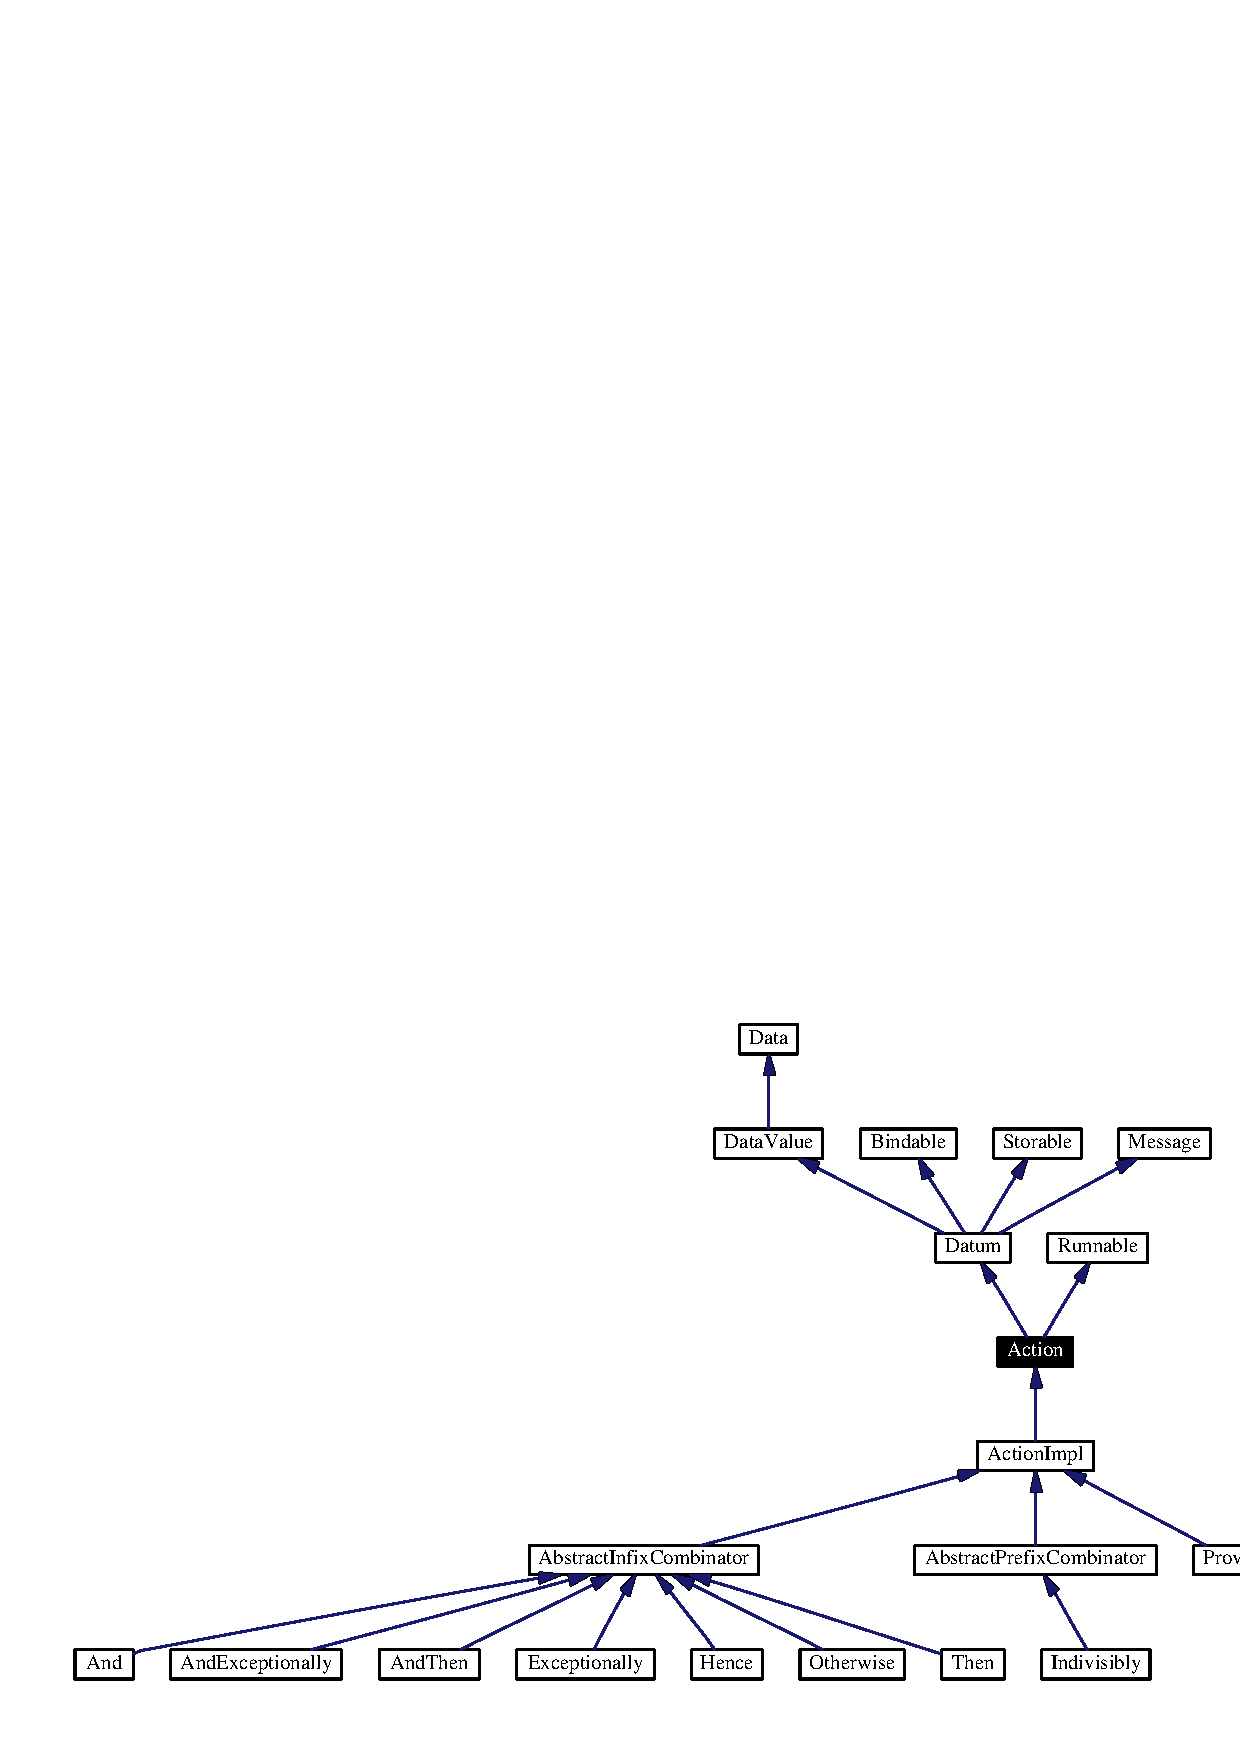
\includegraphics[width=307pt]{interfaceAction__inherit__graph}
\end{center}
\end{figure}
Collaboration diagram for Action:\begin{figure}[H]
\begin{center}
\leavevmode
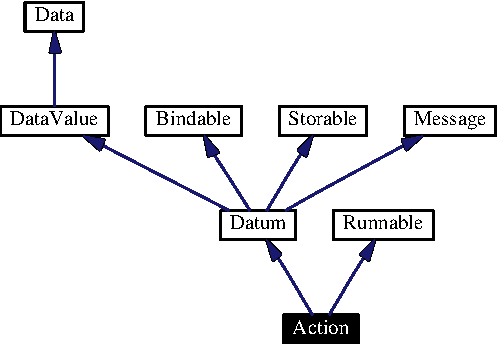
\includegraphics[width=137pt]{interfaceAction__coll__graph}
\end{center}
\end{figure}
\subsection*{Public Methods}
\begin{CompactItemize}
\item 
\hyperlink{interfaceEnactable}{Enactable} \hyperlink{interfaceAction_a0}{enactable\-Value} ()
\item 
\hyperlink{interfaceData}{Data} \hyperlink{interfaceAction_a1}{enact} () throws \hyperlink{classExceptional}{Exceptional}, \hyperlink{classFailed}{Failed}, \hyperlink{classUnfold}{Unfold}
\item 
Action \hyperlink{interfaceAction_a2}{then} (Action action)
\item 
Action \hyperlink{interfaceAction_a3}{and\-Then} (Action action)
\item 
Action \hyperlink{interfaceAction_a4}{and} (Action action)
\item 
Action \hyperlink{interfaceAction_a5}{exceptionally} (Action action)
\item 
Action \hyperlink{interfaceAction_a6}{and\-Exceptionally} (Action action)
\item 
Action \hyperlink{interfaceAction_a7}{otherwise} (Action action)
\item 
Action \hyperlink{interfaceAction_a8}{hence} (Action action)
\item 
Action \hyperlink{interfaceAction_a9}{indivisibly} ()
\end{CompactItemize}


\subsection{Member Function Documentation}
\hypertarget{interfaceAction_a4}{
\index{Action@{Action}!and@{and}}
\index{and@{and}!Action@{Action}}
\subsubsection[and]{\setlength{\rightskip}{0pt plus 5cm}Action Action::and (Action {\em action})}}
\label{interfaceAction_a4}




Reimplemented in \hyperlink{classActionImpl_a14}{Action\-Impl}.\hypertarget{interfaceAction_a6}{
\index{Action@{Action}!andExceptionally@{andExceptionally}}
\index{andExceptionally@{andExceptionally}!Action@{Action}}
\subsubsection[andExceptionally]{\setlength{\rightskip}{0pt plus 5cm}Action Action::and\-Exceptionally (Action {\em action})}}
\label{interfaceAction_a6}




Reimplemented in \hyperlink{classActionImpl_a16}{Action\-Impl}.\hypertarget{interfaceAction_a3}{
\index{Action@{Action}!andThen@{andThen}}
\index{andThen@{andThen}!Action@{Action}}
\subsubsection[andThen]{\setlength{\rightskip}{0pt plus 5cm}Action Action::and\-Then (Action {\em action})}}
\label{interfaceAction_a3}




Reimplemented in \hyperlink{classActionImpl_a13}{Action\-Impl}.\hypertarget{interfaceAction_a1}{
\index{Action@{Action}!enact@{enact}}
\index{enact@{enact}!Action@{Action}}
\subsubsection[enact]{\setlength{\rightskip}{0pt plus 5cm}\hyperlink{interfaceData}{Data} Action::enact ()}}
\label{interfaceAction_a1}




Reimplemented in \hyperlink{classActionImpl_a1}{Action\-Impl}, and \hyperlink{classActionImpl_a11}{Action\-Impl}.

Referenced by Action\-Impl::run().

\hypertarget{interfaceAction_a0}{
\index{Action@{Action}!enactableValue@{enactableValue}}
\index{enactableValue@{enactableValue}!Action@{Action}}
\subsubsection[enactableValue]{\setlength{\rightskip}{0pt plus 5cm}\hyperlink{interfaceEnactable}{Enactable} Action::enactable\-Value ()}}
\label{interfaceAction_a0}




Reimplemented in \hyperlink{classActionImpl_a10}{Action\-Impl}.

Referenced by Action\-Impl::and(), Action\-Impl::and\-Exceptionally(), Action\-Impl::and\-Then(), Action\-Impl::exceptionally(), Action\-Impl::hence(), Action\-Impl::otherwise(), and Action\-Impl::then().

\hypertarget{interfaceAction_a5}{
\index{Action@{Action}!exceptionally@{exceptionally}}
\index{exceptionally@{exceptionally}!Action@{Action}}
\subsubsection[exceptionally]{\setlength{\rightskip}{0pt plus 5cm}Action Action::exceptionally (Action {\em action})}}
\label{interfaceAction_a5}




Reimplemented in \hyperlink{classActionImpl_a15}{Action\-Impl}.\hypertarget{interfaceAction_a8}{
\index{Action@{Action}!hence@{hence}}
\index{hence@{hence}!Action@{Action}}
\subsubsection[hence]{\setlength{\rightskip}{0pt plus 5cm}Action Action::hence (Action {\em action})}}
\label{interfaceAction_a8}




Reimplemented in \hyperlink{classActionImpl_a18}{Action\-Impl}.\hypertarget{interfaceAction_a9}{
\index{Action@{Action}!indivisibly@{indivisibly}}
\index{indivisibly@{indivisibly}!Action@{Action}}
\subsubsection[indivisibly]{\setlength{\rightskip}{0pt plus 5cm}Action Action::indivisibly ()}}
\label{interfaceAction_a9}




Reimplemented in \hyperlink{classActionImpl_a19}{Action\-Impl}.\hypertarget{interfaceAction_a7}{
\index{Action@{Action}!otherwise@{otherwise}}
\index{otherwise@{otherwise}!Action@{Action}}
\subsubsection[otherwise]{\setlength{\rightskip}{0pt plus 5cm}Action Action::otherwise (Action {\em action})}}
\label{interfaceAction_a7}




Reimplemented in \hyperlink{classActionImpl_a17}{Action\-Impl}.\hypertarget{interfaceAction_a2}{
\index{Action@{Action}!then@{then}}
\index{then@{then}!Action@{Action}}
\subsubsection[then]{\setlength{\rightskip}{0pt plus 5cm}Action Action::then (Action {\em action})}}
\label{interfaceAction_a2}




Reimplemented in \hyperlink{classActionImpl_a12}{Action\-Impl}.

The documentation for this interface was generated from the following file:\begin{CompactItemize}
\item 
\hyperlink{Action_8java-source}{Action.java}\end{CompactItemize}
